\chapter{Calibraci\'{o}n}
\label{chap:calibracion}
\epigraph{On two occasions I have been asked, ‘If you put into the machine wrong figures, will the right answers come out?’  I am not able rightly to apprehend the kind of confusion of ideas that could provoke such a question.}{Charles Babbage}

En este cap\'{i}tulo se brinda una descripci\'{o}n del proceso utilizado para la calibraci\'{o}n del experimento. Primero se describe el modelo de c\'{a}mara utilizado en la t\'{e}cnica propuesta. Seguidamente, se detalla el algoritmo utilizado para obtener los par\'{a}metros intr\'{i}nsecos y extr\'{i}nsecos de la c\'{a}mara. Posteriormente, se detalla el algoritmo utilizado para calcular los elementos de rotaci\'{o}n y traslaci\'{o}n entre c\'{a}maras. Finalmente se describe el proceso para estimar la matriz fundamental y la matriz esencial de la c\'{a}mara. Cabe destacar que lograr una buena calibraci\'{o}n es de suma importancia dado que afecta considerablemente el resultado final de la reconstrucci\'{o}n.


\section{Modelo de c\'{a}mara}
Una c\'{a}mara es un mapeo entre el mundo 3D (espacio del objeto) y una imagen 2D. El modelo m\'{a}s b\'{a}sico de este mapeo es la c\'{a}mara \textit{\textbf{pinhole}} la cual no posee lente y puede ser construida utilizando una caja con una peque\~na abertura en uno de sus lados, como se muestra en la figura ~\ref{fig:Pinhole1}. La luz que rebota sobre la escena pasa \'{u}nicamente a trav\'{e}s de la abertura y proyecta una imagen invertida en la parte opuesta de la caja (plano proyectivo). 


\begin{figure}[H]
\centering
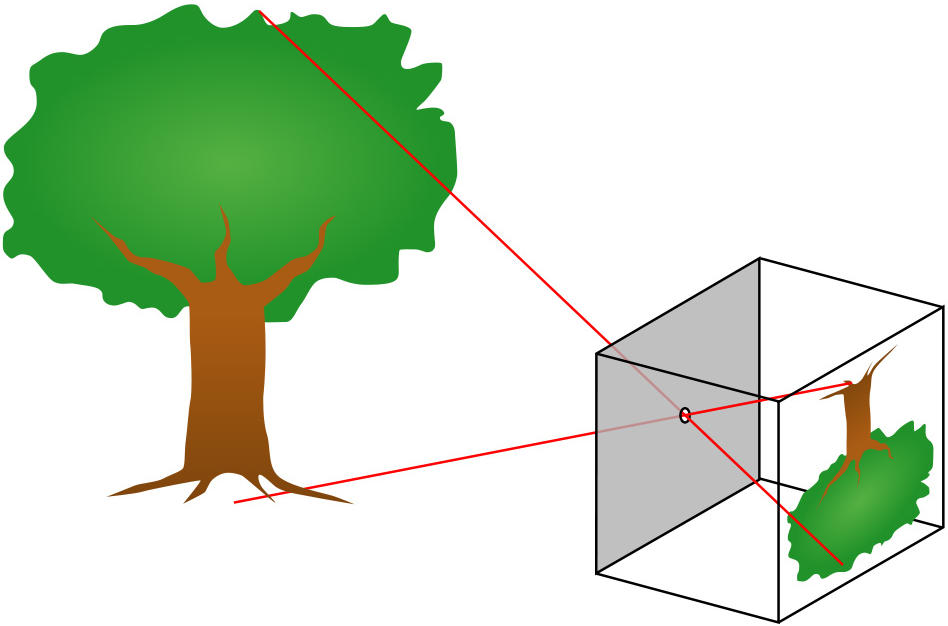
\includegraphics[width=0.8\textwidth]{images/pinhole1.png}
\caption[Modelo b\'{a}sico de c\'{a}mara \textit{pinhole}]%
{Los rayos de luz que rebotan sobre un objeto pasan a trav\'{e}s de un peque\~no agujero para formar una imagen invertida en el plano proyectivo. Imagen tomada del sitio \url{http://mediainfotain.blogspot.com/2010/08/types-of-camera.html} \copyright}
\label{fig:Pinhole1}
\end{figure}


De acuerdo con \cite{Hartley_Zisserman_2003,Faugeras_Luong_2001}, la geometr\'{i}a de esta c\'{a}mara asume que las coordenadas de la imagen son coordenadas Euclidianas con escalas iguales en ambas direcciones (\textit{x}, \textit{y}) como se muestra en la figura ~\ref{fig:Pinhole2}. Para el caso de c\'{a}maras \ac{CCD}, existe la posibilidad de tener pixeles no cuadrados. Si las coordenadas de la imagen se miden en pixeles, existe el efecto extra de introducir factores de escala desiguales en cada direcci\'{o}n. Afortunadamente, existe una variaci\'{o}n del modelo b\'{a}sico que permite determinar la transformaci\'{o}n entre coordenadas del mundo real a coordenadas de pixeles de la imagen.


\begin{figure}[H]
\centering
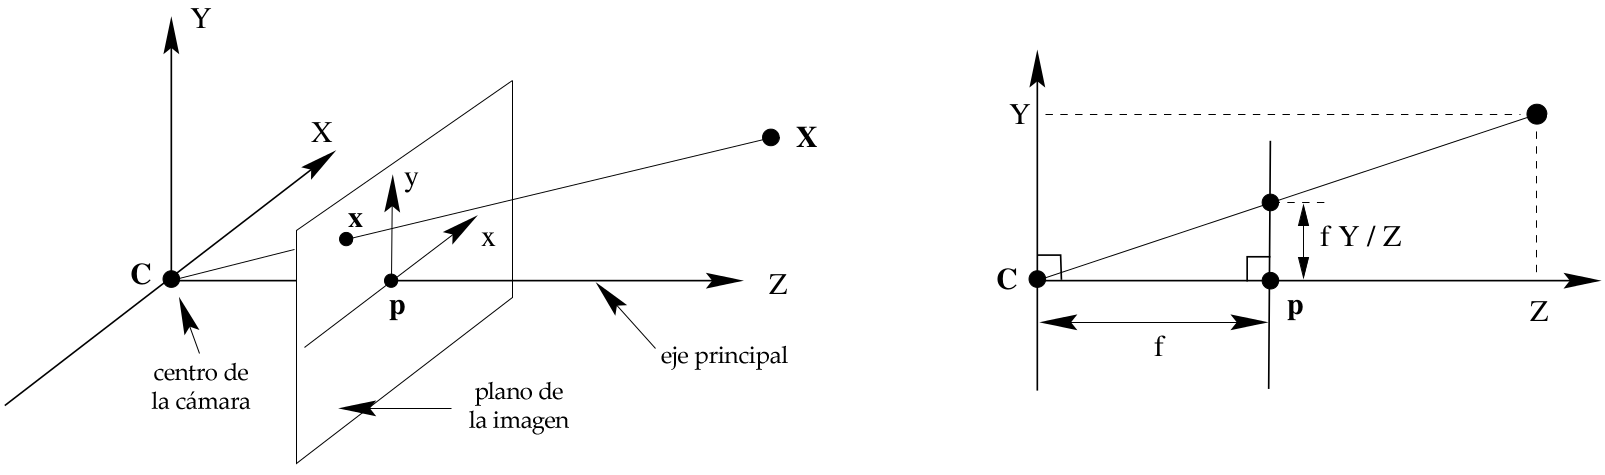
\includegraphics[width=1.0\textwidth]{images/pinhole.png}
\caption[Geometr\'{i}a de la c\'{a}mara \textit{pinhole}]%
{\textbf{C} es el centro de la c\'{a}mara y \textbf{p} el punto principal. El centro de la c\'{a}mara se posiciona justo en el origen de las coordenadas. N\'{o}tese que el plano de la imagen se posiciona frente al centro de la c\'{a}mara. Imagen tomada del libro \textit{Multiple View Geometry} de Richard Hartley y Andrew Zisserman \copyright \cite{Hartley_Zisserman_2003}.}
\label{fig:Pinhole2}
\end{figure}


Seg\'{u}n \cite{Szeliski_2010,Shah_1983}, la calibraci\'{o}n es el proceso de encontrar los valores \textit{verdaderos} de una c\'{a}mara que produce determinada fotograf\'{i}a o video. Usualmente, los par\'{a}metros de la c\'{a}mara son representados en la \textit{matriz de la c\'{a}mara} y los valores de distorsi\'{o}n son representados en la \textit{matriz de coeficientes de distorsi\'{o}n}. El algoritmo de calibraci\'{o}n del sistema de captura utilizado para la t\'{e}cnica de reconstrucci\'{o}n se basa en el modelo b\'{a}sico de c\'{a}mara \textit{pinhole} con proyecci\'{o}n perspectiva, como se indica en \cite{Hartley_Zisserman_2003}, en el cual la matriz de proyecci\'{o}n \textit{P} de la c\'{a}mara tiene la forma:

\begin{center}
\vspace{5 mm}
$
\textbf{\textit{P}} = \textbf{\textit{K}}[\textbf{\textit{R}}|\textbf{\textit{-Rt}}] con \textbf{\textit{K}} = 
\left[ {
\begin{array}{*{20}c}
   c_x & h_s & h_x  \\
   0   & c_y & h_y  \\
   0   & 0   & 1    \\
\end{array} 
} \right]
$
\vspace{5 mm}
\end{center}

donde \textit{\textbf{R}} indica la rotaci\'{o}n de la c\'{a}mara, \textit{\textbf{t}} es la posici\'{o}n del centro proyectivo en coordenadas del mundo real, \textit{\textbf{K}} contiene los par\'{a}metros internos de la c\'{a}mara: \textit{$c_x$} y \textit{$c_y$} son la longitud horizontal y vertical del foco (en pixeles), \textit{\textbf{h}} = $[h_x,h_y]^T$ es el punto principal de la imagen y \textit{$h_s$} es la medida de la inclinaci\'{o}n de la imagen (\textit{skew}). Afortunadamente, la matriz \textbf{\textit{K}} puede ser f\'{a}cilmente calculada utilizando la t\'{e}cnica de calibraci\'{o}n con tablero.

\section{Estimaci\'{o}n de K usando calibraci\'{o}n con tablero}
Por muchos a\~nos, la estimaci\'{o}n de los par\'{a}metros intr\'{i}nsecos y extr\'{i}nsecos de la c\'{a}mara ha sido un tema de gran inter\'{e}s para los investigadores del \'{a}rea de la visi\'{o}n artificial debido a que usualmente precede al proceso de reconstrucci\'{o}n de la profundidad \cite{Cyganek_Siebert_2009,Maybank_Faugeras_1992,Tsai_R_Y_1987}.

Una gran parte del inter\'{e}s ha sido dedicado al desarrollo de t\'{e}cnicas de calibraci\'{o}n r\'{a}pidas para c\'{a}maras simples, como es el caso de \cite{Zhang_camcal_2004} el cual propone un m\'{e}todo de calibraci\'{o}n de c\'{a}maras utilizando patrones gr\'{a}ficos.

La calibraci\'{o}n con tablero es una de las t\'{e}cnicas m\'{a}s populares en el \'{a}rea de la visi\'{o}n artificial por su relativa facilidad de implementaci\'{o}n y por su precisi\'{o}n en cuanto a los resultados \cite{Szeliski_2010, Tsai_R_Y_1987}. Para realizar la calibraci\'{o}n, se procede a presentar ante la c\'{a}mara un patr\'{o}n similar al de un tablero de ajedrez, con el cual es posible estimar con gran precisi\'{o}n la orientaci\'{o}n relativa y los par\'{a}metros intr\'{i}nsecos de la c\'{a}mara. El proceso calcula una m\'{e}trica Euclidiana con escala absoluta en el sistema de coordenadas de referencia de la calibraci\'{o}n \cite{Jahne_Haubecker_Ray_2002}, a partir de la cual es posible obtener la matriz de la c\'{a}mara \textbf{\textit{K}} y la matriz de coeficientes de distorsi\'{o}n. En la figura ~\ref{fig:ACalibration1} se muestra la ejecuci\'{o}n del algoritmo de calibraci\'{o}n con tablero utilizado durante el experimento.


\begin{figure}[H]
\centering
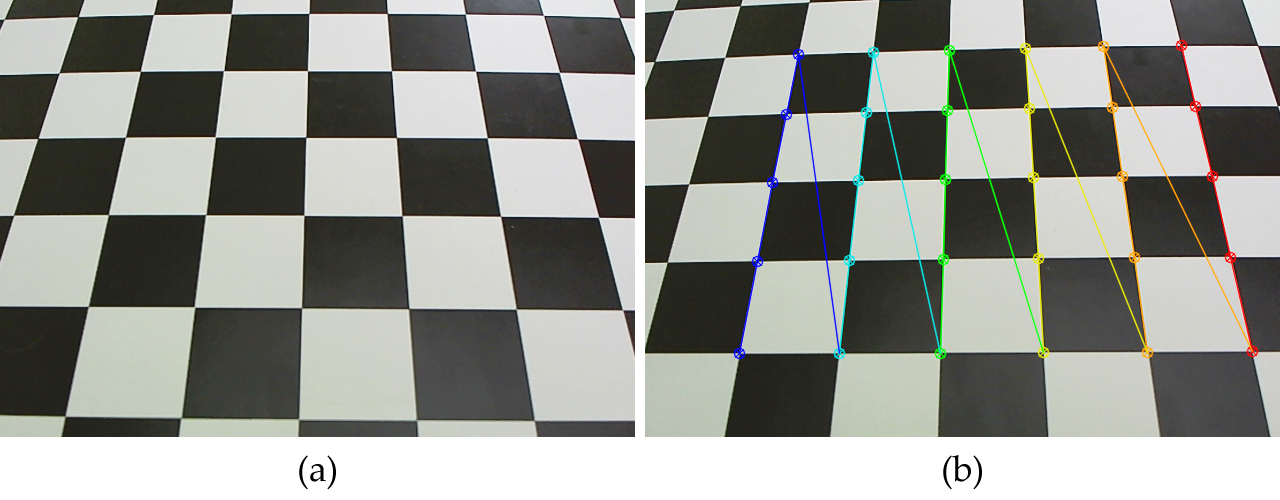
\includegraphics[width=1.0\textwidth]{images/acalibration0.png}
\caption[Calibraci\'{o}n usando tablero]%
{\textbf{(a)} Se presenta un patr\'{o}n de un tablero con un n\'{u}mero predeterminado de filas y columnas al algoritmo de calibraci\'{o}n. \textbf{(b)} El algoritmo calcula con gran precisi\'{o}n, a partir de los cuadros encontrados, la orientaci\'{o}n relativa as\'{i} como los valores intr\'{i}nsecos de la c\'{a}mara los cuales son necesarios para las siguientes etapas de la reconstrucci\'{o}n. Im\'{a}genes generadas por el autor de este documento.}
\label{fig:ACalibration1}
\end{figure}


\section{Estimaci\'{o}n del movimiento entre c\'{a}maras}
Una vez obtenida la matriz \textbf{\textit{K}} se procede a estimar el movimiento de la c\'{a}mara a partir de un par de im\'{a}genes estereosc\'{o}picas. Una c\'{a}mara\footnote{Con tal de simplificar la descripci\'{o}n de la t\'{e}cnica propuesta, se refiere a c\'{a}mara como la representaci\'{o}n de una vista (imagen) y no al aparato en s\'{i}.} tiene una posici\'{o}n en el espacio tridimensional y una direcci\'{o}n de la vista. Entre dos c\'{a}maras, existe un elemento de traslaci\'{o}n (matriz \textit{\textbf{t}}) y uno de rotaci\'{o}n (matriz \textit{\textbf{R}}) de la direcci\'{o}n de la vista, los cuales son necesarios para el proceso de la reconstrucci\'{o}n \cite{Faugeras_Luong_2001,Hartley_Zisserman_2003,Faugeras_1993}. En la figura ~\ref{fig:CameraMotion1} se muestra el movimiento de la c\'{a}mara entre pares de im\'{a}genes estereosc\'{o}picas.


\begin{figure}[H]
\centering
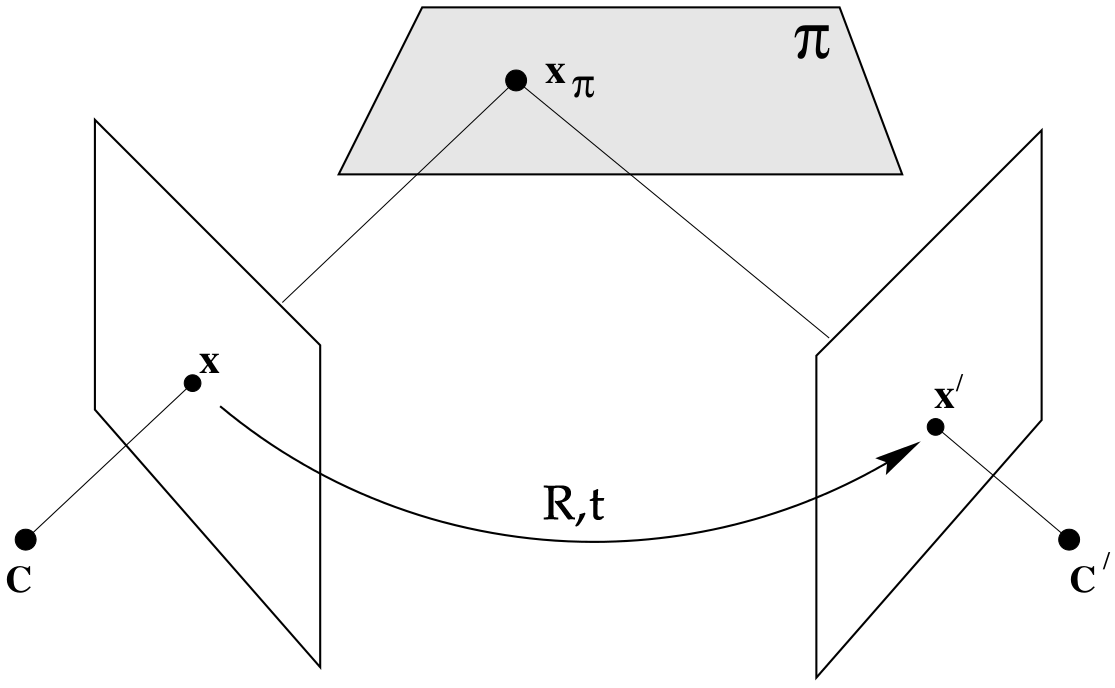
\includegraphics[width=1.0\textwidth]{images/camera-rt1.png}
\caption[Movimiento de c\'{a}mara entre pares de im\'{a}genes estereosc\'{o}picas]%
{La c\'{a}mara es indicada por su centro \textbf{C} en la primera posici\'{o}n en el espacio tridimensional y \textbf{C'} en la siguiente posici\'{o}n. Existe un elemento de rotaci\'{o}n \textbf{\textit{R}} y traslaci\'{o}n \textbf{\textit{t}} entre \textbf{C} y \textbf{C'} en pares de im\'{a}genes estereosc\'{o}picas. Imagen tomada del libro \textit{Multiple View Geometry} de Richard Hartley y Andrew Zisserman \copyright \cite{Hartley_Zisserman_2003}.}
\label{fig:CameraMotion1}
\end{figure}


En un aparejo est\'{e}reo (del ingl\'{e}s \textit{stereo rig}), el movimiento de traslaci\'{o}n y rotaci\'{o}n entre las c\'{a}maras se asume conocido \cite{Faugeras_Toscani_1986,Hartley_Zisserman_2003}. Tal es el caso de la c\'{a}mara estereosc\'{o}pica Minoru. La distancia entre sus dos c\'{a}maras puede ser calculada con precisi\'{o}n y as\'{i} evitar recalcularla para cada par de im\'{a}genes estereosc\'{o}picas tomadas con esta c\'{a}mara. Sin embargo, utilizar aparejos est\'{e}reo para realizar reconstrucci\'{o}n tridimensional tiene sus limitaciones pr\'{a}cticas y est\'{a} fuera del alcance de este trabajo. La t\'{e}cnica propuesta se basa en reconstrucci\'{o}n monocular (una c\'{a}mara). Es por esto que durante el experimento s\'{o}lo se utiliz\'{o} una de las dos c\'{a}maras de Minoru para la captura de las im\'{a}genes.

Dos im\'{a}genes (sean \textit{\textbf{I}} y \textit{\textbf{D}}) de un mismo objeto desde posiciones no muy diferentes en el espacio tridimensional (posiciones \textit{\textbf{a}} y \textit{\textbf{b}}) tomadas por una misma c\'{a}mara, son geom\'{e}tricamente equivalentes a tomar la imagen \textit{\textbf{I}} desde la posici\'{o}n \textit{\textbf{a}} con una c\'{a}mara y luego tomar la imagen \textit{\textbf{D}} desde la posici\'{o}n \textit{\textbf{b}} con una segunda c\'{a}mara. Esto significa que si se detecta una serie de puntos clave (del ingl\'{e}s \textit{keypoints}) en la imagen \textit{\textbf{I}} y luego se encuentran esos mismos puntos clave en la imagen \textit{\textbf{D}}, es posible determinar la traslaci\'{o}n \textit{t} y rotaci\'{o}n \textit{R} de las c\'{a}maras. Se puede determinar cu\'{a}nto y c\'{o}mo se ha movido un pixel entre una imagen y otra por medio de la estimaci\'{o}n de un mapa de movimiento (del ingl\'{e}s \textit{motion map}).

Cabe destacar que para la t\'{e}cnica propuesta es indiferente si procesa pares de im\'{a}genes provenientes de un aparejo est\'{e}reo o si procesa secuencias de im\'{a}genes provenientes de un sistema monocular como el utilizado.


\section{Mapa de movimiento}
Existen diferentes formas de obtener un mapa de movimiento. Algunas t\'{e}cnicas se basan en la detecci\'{o}n de l\'{i}neas \cite{Ding_Goshtasby_2001}, detecci\'{o}n de esquinas \cite{Harris_Stephens_1988}, detecci\'{o}n de \textit{blobs\footnote{En la visi\'{o}n artificial, la detecci\'{o}n de \textit{blobs} se refiere a los m\'{e}todos matem\'{a}ticos cuyo objetivo es detectar regiones en im\'{a}genes digitales que difieren en propiedades, tales como color o brillo, en comparaci\'{o}n con las \'{a}reas que se encuentran alderedor de esas regiones.}} \cite{Ming_Huadong_2007}, entre otras. 

Una de las t\'{e}cnicas m\'{a}s utilizadas en el campo de la visi\'{o}n artificial es el pareo entre caracter\'{i}sticas sobresalientes\footnote{Puntos clave y las caracter\'{i}sticas sobresalientes se refieren al mismo concepto.} (del ingl\'{e}s \textit{rich feature matching}). Lo que se hace es detectar en cada par de im\'{a}genes estereosc\'{o}picas un grupo de caracter\'{i}sticas sobresalientes con las cuales calcular descriptores invariantes para posteriormente realizar un pareo entre los grupos de cada imagen \cite{Shapiro_Stockman_2001,Szeliski_2010,Cyganek_Siebert_2009}.

Existe una cantidad considerable de algoritmos para la detecci\'{o}n de caracter\'{i}sticas sobresalientes, SIFT (del ingl\'{e}s \textit{scale-invariant feature transform}) \cite{Lowe_1999}, SURF (del ingl\'{e}s \textit{speeded up robust features}) \cite{Bay_Ess_Tuytelaars_Vangool_2008}, BRISK (del ingl\'{e}s \textit{binary robust invariant scalable keypoints}) \cite{Leutenegger_Chli_Siegwart_2011}, FAST (del ingl\'{e}s \textit{features from accelerated segment test}) \cite{Rosten_Drummond_2006}, HARRIS (por su autor Chris Harris) \cite{Harris_Stephens_1988} y muchos m\'{a}s. En la figura ~\ref{fig:PointDetection1} se muestran pruebas realizadas a cuatro de los algoritmos de detecci\'{o}n de caracter\'{i}sticas sobresalientes: \textit{BRISK}, \textit{DENSE}, \textit{SURF} y \textit{FAST} con pir\'{a}mide.


\begin{figure}[H]
\centering
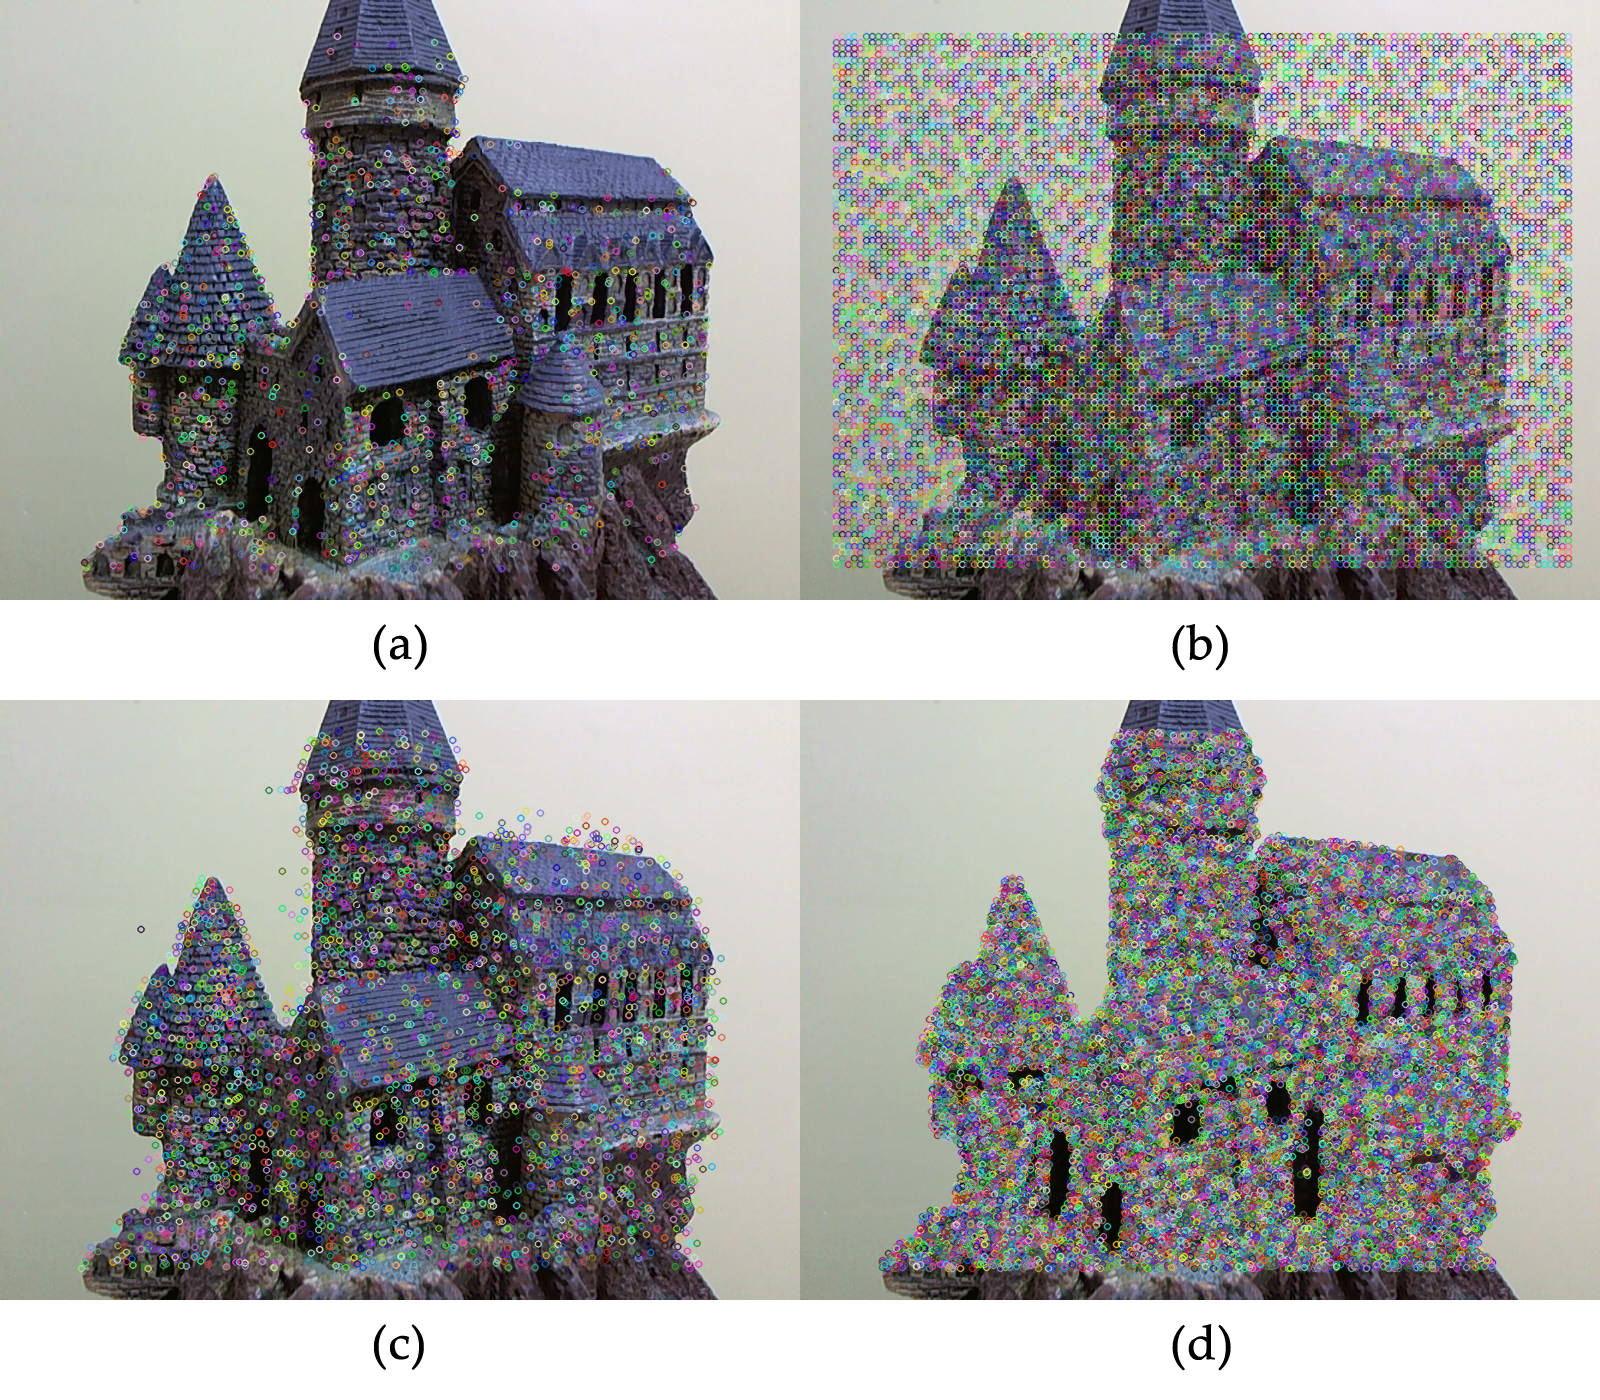
\includegraphics[width=1.0\textwidth]{images/pointdetection1.png}
\caption[Detecci\'{o}n de caracter\'{i}sticas sobresalientes usando BRISK, DENSE, SURF y FAST con pir\'{a}mide]%
{\textbf{(a)} \textit{BRISK} encontr\'{o} un total de 1176 puntos en la imagen. \textbf{(b)} \textit{DENSE} encontr\'{o} un total de 13400 puntos en la imagen. \textbf{(c)} \textit{SURF} encontr\'{o} un total de 3671 puntos en la imagen. \textbf{(d)} \textit{FAST} con pir\'{a}mide encontr\'{o} un total de 17296 puntos en la imagen. N\'{o}tese como \textit{SURF} y \textit{DENSE} detectaron puntos en \'{a}reas de la imagen en las cuales no existe nada sobresaliente mientras que \textit{FAST} con pir\'{a}mide no. La resoluci\'{o}n de la imagen es de 800x600 pixeles. Im\'{a}genes generadas por el autor de este documento.}
\label{fig:PointDetection1}
\end{figure}


De acuerdo con KITTI\footnote{KITTI es un proyecto del \textit{Karlsruhe Institute of Technology} y de \textit{Toyota Technological Institute at Chicago} el cual desarrolla evaluaciones para problemas del mundo real en el \'{a}rea de la visi\'{o}n artificial. Sitio web: \url{http://www.cvlibs.net/datasets/kitti}}, Middleburry\footnote{Middleburry College es una universidad privada ubicada en Middleburry, Vermont - USA. El sitio web \url{http://vision.middlebury.edu} se cre\'{o} como repositorio de evaluaciones y conjuntos de datos relacionados con la visi\'{o}n artificial.} y Computer Vision Talks \footnote{\textit{Computer Vision Talks} es un sitio dedicado a investigaciones en el \'{a}rea de la visi\'{o}n artificial. Sitio web: \url{http://computer-vision-talks.com/2011/01/comparison-of-the-opencvs-feature-detection-algorithms-2}}, \textit{FAST} con pir\'{a}mide, \textit{FAST} y \textit{SURF} son los algoritmos m\'{a}s r\'{a}pidos pero \textit{FAST} con pir\'{a}mide detecta una mayor cantidad de caracter\'{i}sticas, lo cual lo hace candidato adecuado para la t\'{e}cnica propuesta. En \cite{Tuytelaars_Mikolajczyk_2007} se detalla m\'{a}s a fondo c\'{o}mo funciona cada uno de los diferentes algoritmos.

Para la extracci\'{o}n de los descriptores se utiliz\'{o} ORB \cite{Rublee_Rabaud_Konolige_Bradski_2011} por su conocida eficiencia y rapidez en comparaci\'{o}n con algoritmos tradicionales como SIFT o SURF. Finalmente, se utiliz\'{o} un algoritmo de fuerza bruta \textit{BruteForce}, dado que es una de las formas m\'{a}s sencillas de comparar y hacer pareo entre caracter\'{i}sticas. B\'{a}sicamente, compara cada una de las caracter\'{i}sticas de un grupo contra las caracter\'{i}sticas del otro grupo y luego obtiene el mejor pareo entre ambos.

Sin embargo, despu\'{e}s de las diferentes pruebas realizadas se determin\'{o} que a pesar de que todo el proceso de detecci\'{o}n, extracci\'{o}n y pareo de caracter\'{i}sticas es relativamente r\'{a}pido, el mapa de movimiento resultante del pareo es muy disperso (pocos puntos) en la mayor\'{i}a de los casos. Esto provocar\'{i}a que el resultado final de la reconstrucci\'{o}n tridimensional tambi\'{e}n sea disperso. En la figura ~\ref{fig:FeatureMatching1} se muestran pruebas realizadas a tres de los algoritmos de pareo de caracter\'{i}sticas sobresalientes.


\begin{figure}[H]
\centering
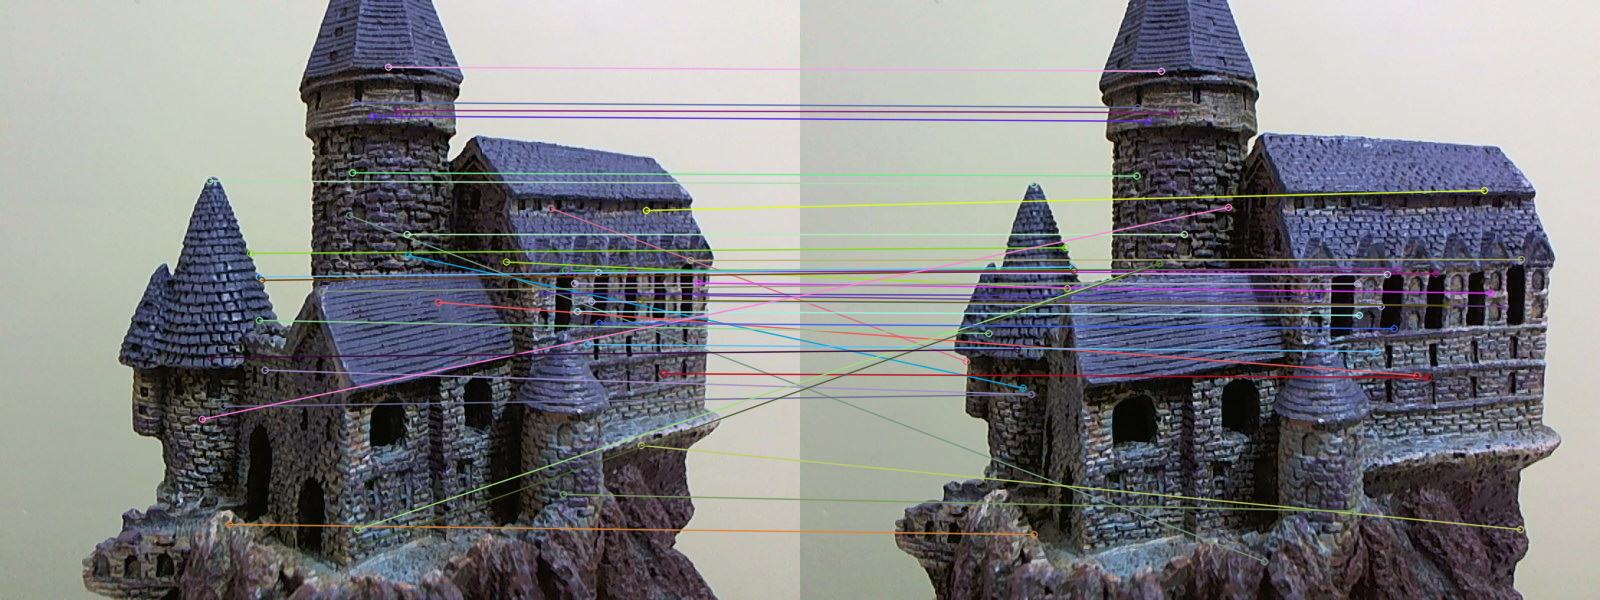
\includegraphics[width=1.0\textwidth]{images/briskmatches1.png}
(a)
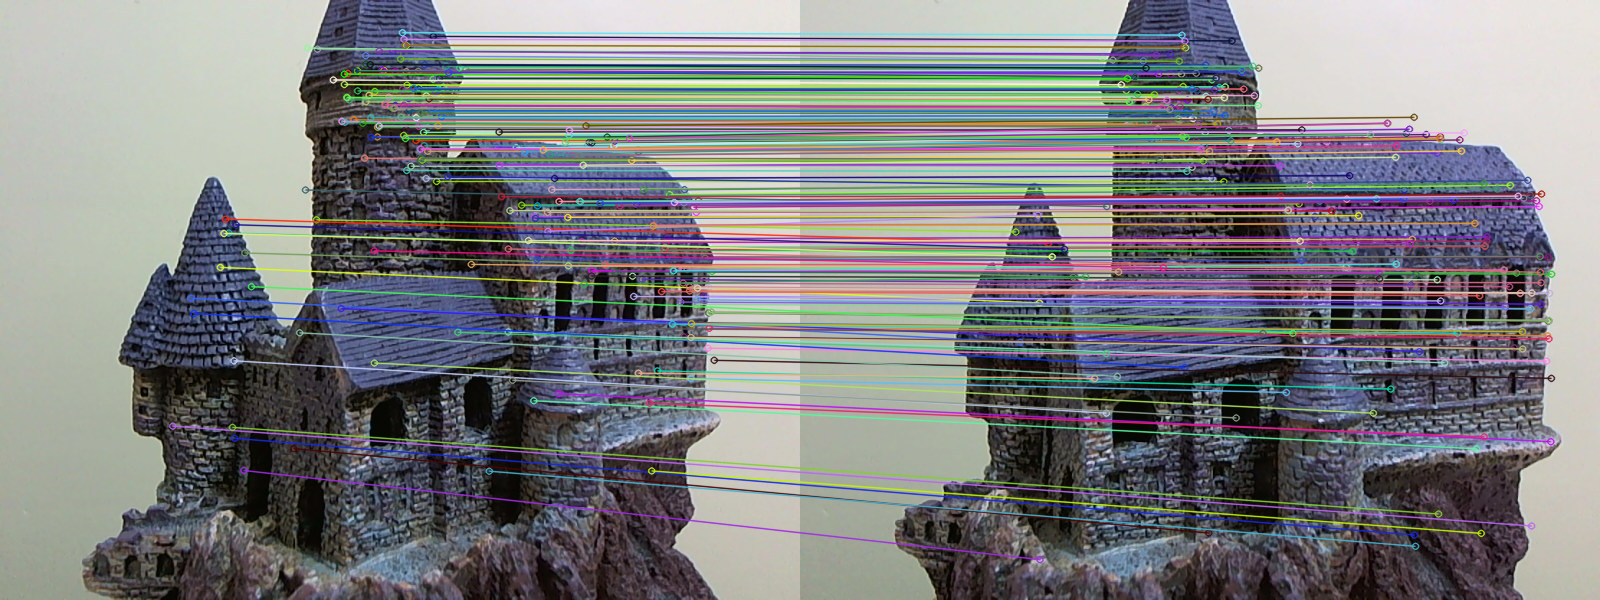
\includegraphics[width=1.0\textwidth]{images/surfmatches1.png}
(b)
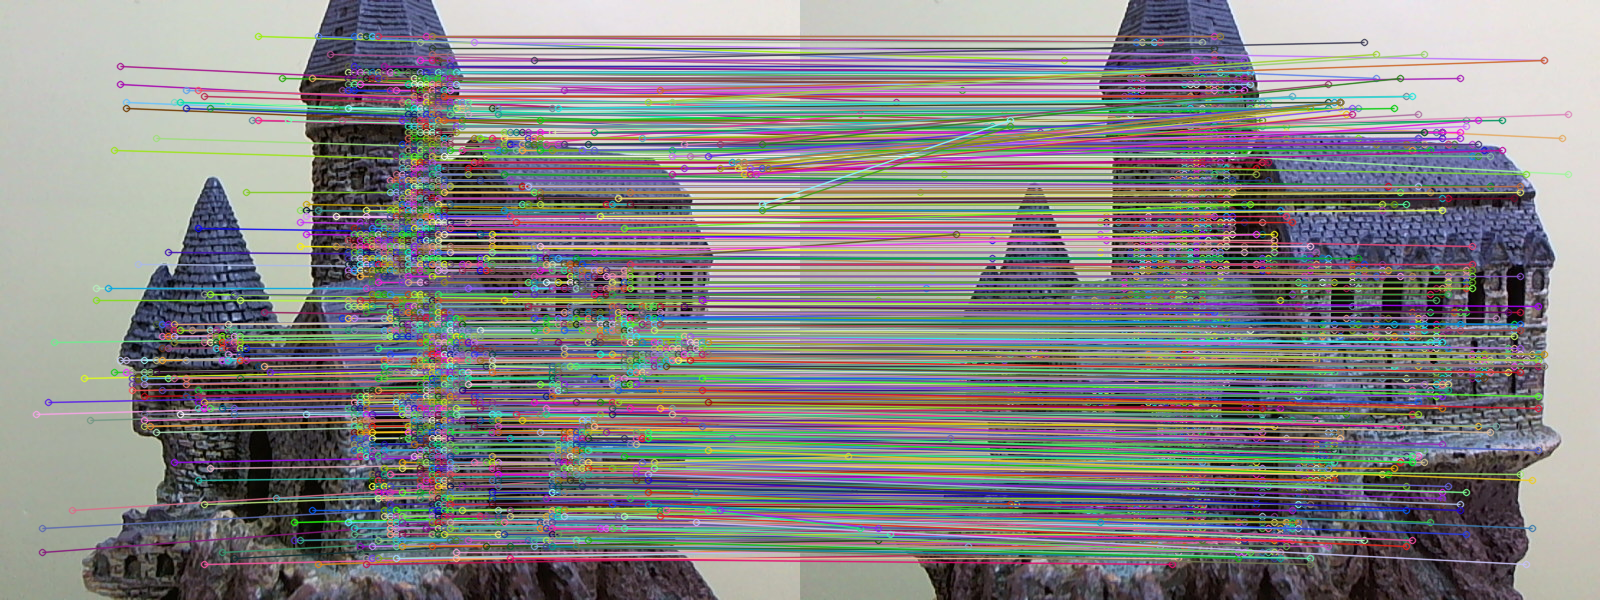
\includegraphics[width=1.0\textwidth]{images/densematches1.png}
(c)
\caption[Pareo de caracter\'{i}sticas y descriptores invariantes usando BRISK, SURF y DENSE]%
{\textbf{(a)} Pareo de caracter\'{i}sticas sobresalientes usando el algoritmo de BRISK. \textbf{(b)} Pareo de caracter\'{i}sticas sobresalientes usando el algoritmo de SURF. \textbf{(c)} Pareo de caracter\'{i}sticas sobresalientes usando el algoritmo de DENSE. N\'{o}tese, como el pareo entre el par de im\'{a}genes estereosc\'{o}picas es bastante disperso y en algunos casos incorrecto. Im\'{a}genes generadas por el autor de este documento.}
\label{fig:FeatureMatching1}
\end{figure}


Como se busca obtener una reconstrucci\'{o}n densa y no una dispersa, se opt\'{o} por desarrollar un algoritmo basado en la detecci\'{o}n del flujo \'{o}ptico (del ingl\'{e}s \textit{optical flow}) \cite{Szeliski_2010,Cyganek_Siebert_2009} en conjunto con una t\'{e}cnica pir\'{a}mide para el preprocesamiento de las im\'{a}genes. Generalmente, la detecci\'{o}n del flujo \'{o}ptico es costosa en tiempo y no apta para ser utilizada en reconstrucci\'{o}n tridimensional r\'{a}pida, dado que hay que rastrear todos y cada uno de los pixeles, pero el m\'{e}todo propuesto se basa en una reciente t\'{e}cnica lineal que es suficientemente r\'{a}pida para la reconstrucci\'{o}n y adicionalmente, permite generar mapas de movimiento densos.

\subsection{Preprocesamiento de im\'{a}genes usando pir\'{a}mide}
El concepto de im\'{a}genes pir\'{a}mide se define como una secuencia de copias de una imagen original en la cual la muestra de densidad y la resoluci\'{o}n han sido disminuidas a pasos regulares, usualmente por un factor de 2 en cada coordenada \cite{Adelson_Anderson_Bergen_Burt_Ogden_1984}. Se busca reducir la cantidad de informaci\'{o}n contenida en la imagen sin que se degrade su calidad durante el procesamiento.

Dos de las t\'{e}cnicas m\'{a}s utilizadas de im\'{a}genes pir\'{a}mide son pir\'{a}mide \textit{Gaussian} y pir\'{a}mide \textit{Laplacian}. La t\'{e}cnica de pir\'{a}mide Gaussian se utiliza para reducir la informaci\'{o}n contenida en las im\'{a}genes mientras que la t\'{e}cnica pir\'{a}mide Laplacian se utiliza para reconstruir una imagen interpolada a partir de una imagen inferior de la pir\'{a}mide (con menor resoluci\'{o}n) \cite{Burt198120,burt_adelson_1095851}.


\begin{figure}[H]
\centering
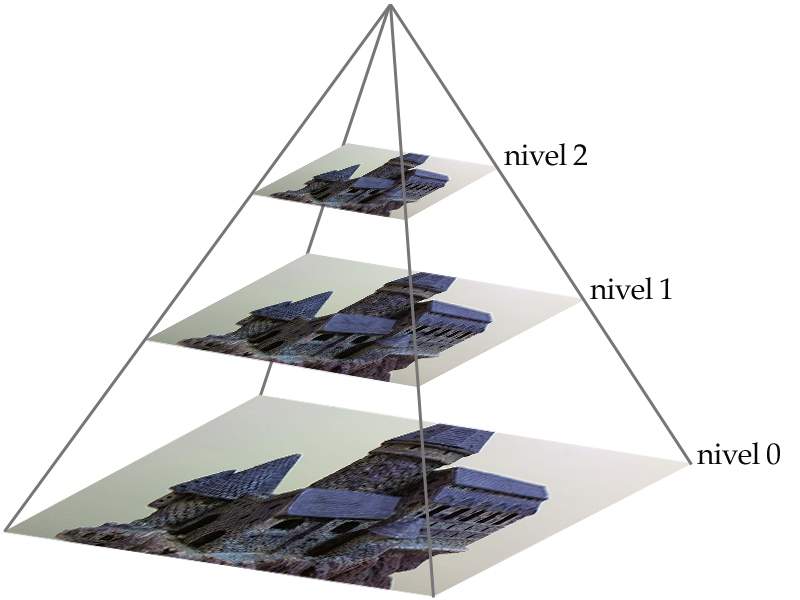
\includegraphics[width=0.75\textwidth]{images/pyramid.png}
\caption[Preprocesamiento de im\'{a}genes usando pir\'{a}mide]%
{En el nivel 0 se encuentra la imagen original con una resoluci\'{o}n de 800x600 lo cual equivale a una cantidad de 480000 pixeles. El nivel 1 muestra la misma imagen reducida a 640x480 con una cantidad de 307200 pixeles y finalmente, la imagen en el nivel 2 con una resoluci\'{o}n de 512x384 equivalente a una cantidad de 196608 pixeles. La reducci\'{o}n en la cantidad de pixeles entre la imagen original y la imagen en el nivel 2 es de un 40.96\%. Imagen generada por el autor de este documento.}
\label{fig:Pyramid}
\end{figure}


Para la t\'{e}cnica propuesta, cada imagen es preprocesada utilizando pir\'{a}mide Gaussian con un factor 2 para reducir la cantidad de informaci\'{o}n que se procesar\'{a} durante la fase de detecci\'{o}n del flujo \'{o}ptico\footnote{La escogencia del factor se realiz\'{o} de forma emp\'{i}rica basada en las diferentes investigaciones y pruebas realizadas pero la t\'{e}cnica no se encuentra limitada por este factor.}. Esto permite mantener bajo el tiempo global de la reconstrucci\'{o}n cuando se utilicen im\'{a}genes de gran resoluci\'{o}n sin afectar considerablemente su calidad. En la figura ~\ref{fig:Pyramid} se muestran un ejemplo de la t\'{e}cnica pir\'{a}mide Gaussian aplicada a una de las im\'{a}genes capturadas durante el experimento.


\subsection{R\'{a}pida detecci\'{o}n del flujo \'{o}ptico}
El primero en introducir este concepto fue el psic\'{o}logo James J. Gibson en 1940 y lo describe como \textit{el est\'{i}mulo visual dotado a los animales que se mueven a trav\'{e}s de la Tierra} \cite{Gibson_1950}. En el \'{a}rea de la visi\'{o}n artificial, el flujo \'{o}ptico trabaja rastreando todos y cada uno de los pixeles de la primera imagen en la segunda imagen, asumiendo que ambas im\'{a}genes son parte de una secuencia y que se encuentran relativamente cerca una de la otra, con el supuesto de que cada pixel puede moverse solamente dentro de cierta \textit{ventana} en la cual se realizar\'{a} la b\'{u}squeda \cite{Gibson_1950,Shapiro_Stockman_2001,Szeliski_2010,Cyganek_Siebert_2009}.

Entre los algoritmos m\'{a}s populares para la detecci\'{o}n densa\footnote{En este contexto, densa significa que se busca el movimiento de todos y cada uno de los pixeles de la imagen.} del flujo \'{o}ptico se encuentran el de \textit{Lucas-Kanade} \cite{Lucas_Kanade_1981} y m\'{a}s recientemente el de \textit{Gunnar Farnebäck} \cite{Farneback_2003}. Usualmente, la detecci\'{o}n densa es costosa en tiempo pero afortunadamente ambos algoritmos son lo suficientemente r\'{a}pidos para ser utilizados en la reconstrucci\'{o}n tridimensional y han sido implementados en una gran variedad de bibliotecas. De acuerdo con KITTI y Middleburry, el algoritmo de Farnebäck es m\'{a}s r\'{a}pido y posee una menor tasa de error\footnote{V\'{e}ase \url{http://www.cvlibs.net/datasets/kitti/eval_stereo_flow.php}}. En la figura ~\ref{fig:OpticalFlow1} se muestra el resultado de una de las pruebas de detecci\'{o}n del flujo \'{o}ptico utilizando el algoritmo de Lucas-Kanade y el de Farnebäck.


\begin{figure}[H]
\centering
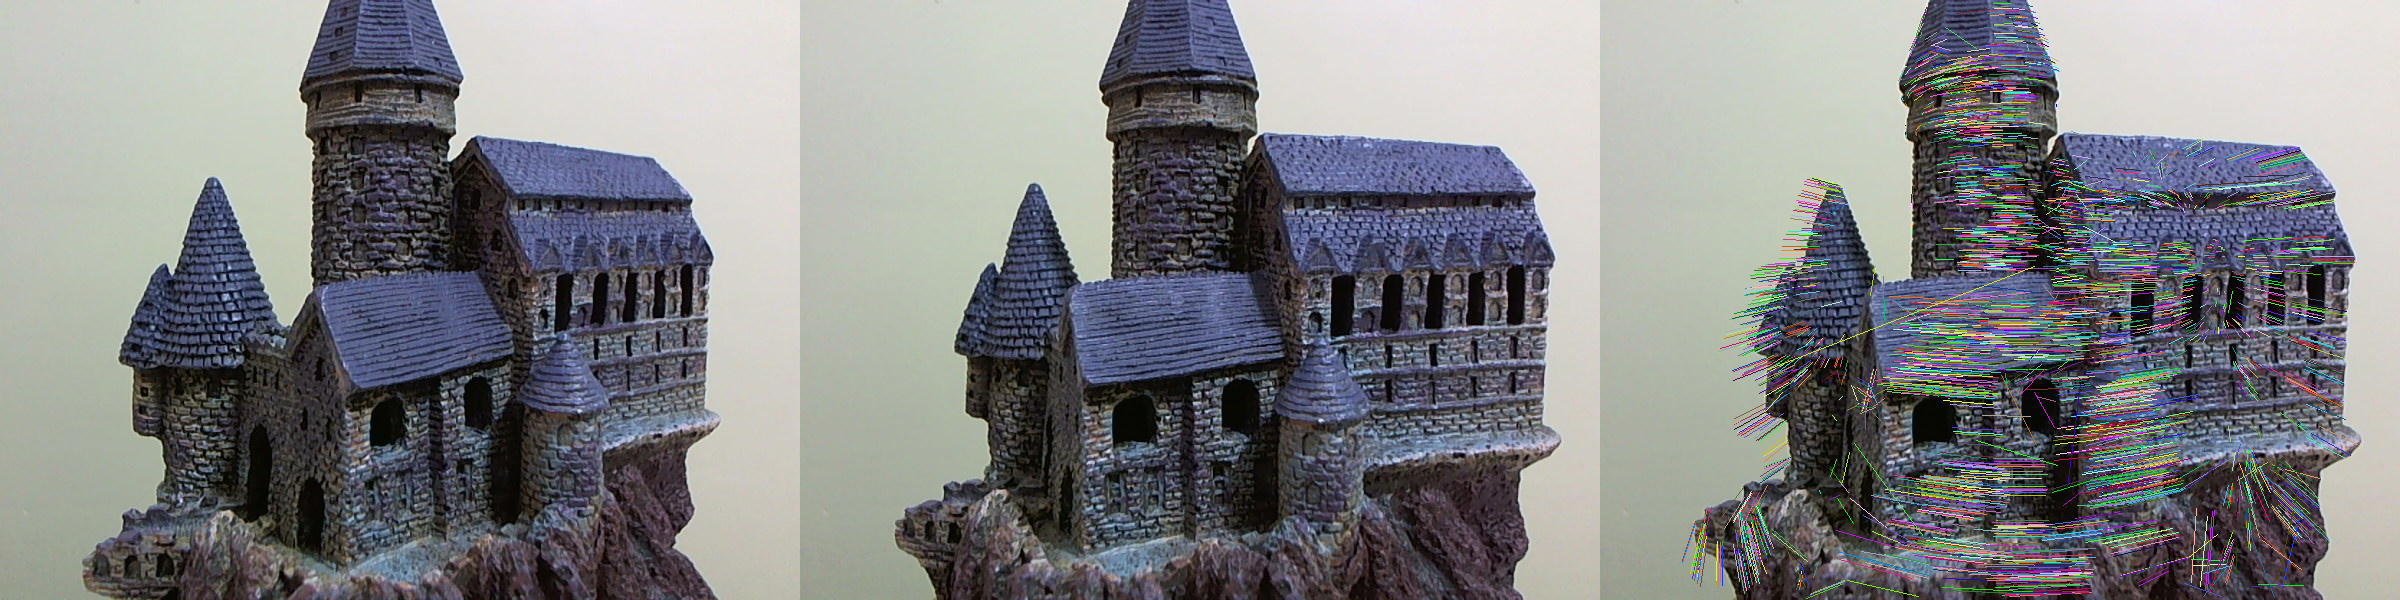
\includegraphics[width=1.0\textwidth]{images/oflucaskanade1.png}
(a)
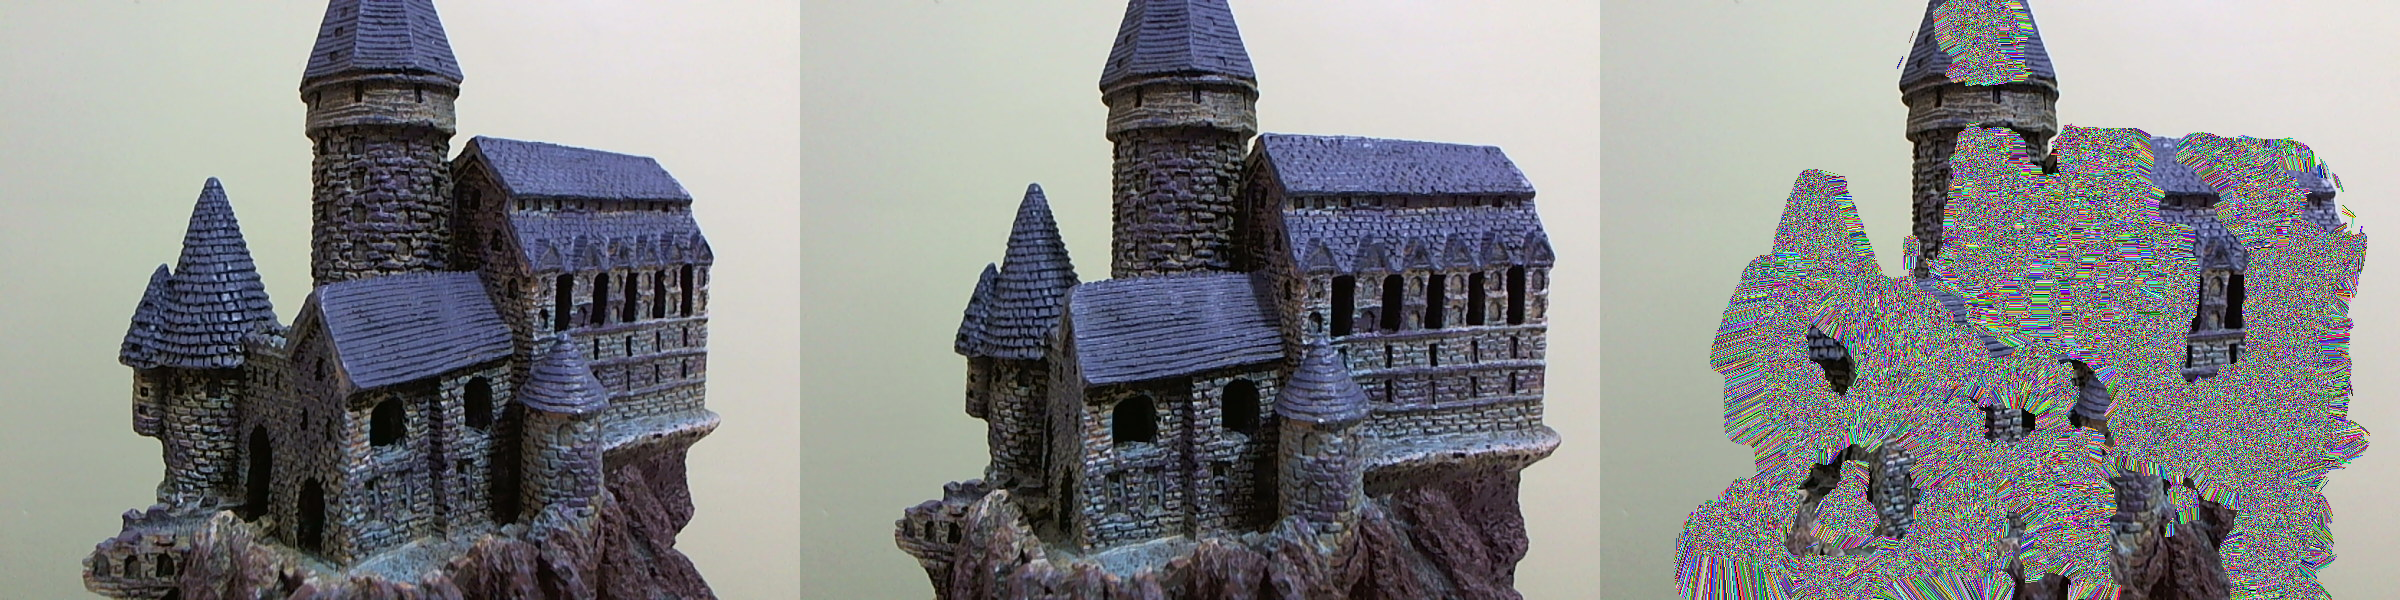
\includegraphics[width=1.0\textwidth]{images/offarneback1.png}
(b)
\caption[Detecci\'{o}n del flujo \'{o}ptico]%
{\textbf{(a)} Detecci\'{o}n densa del flujo \'{o}ptico utilizando el algoritmo de Lucas-Kanade. \textbf{(b)} Detecci\'{o}n densa del flujo \'{o}ptico utilizando el algoritmo de Gunnar Farnebäck. N\'{o}tese la considerable diferencia entre el flujo detectado por Lucas-Kanade vs. Farnebäck. Ambas t\'{e}cnicas est\'{a}n entre las m\'{a}s populares y ha sido implementadas en una gran variedad de bibliotecas de visi\'{o}n artificial. Im\'{a}genes generadas por el autor de este documento.}
\label{fig:OpticalFlow1}
\end{figure}


Farnebäck permite generar el mapa denso de movimiento requerido para la calibraci\'{o}n. Sin embargo, pruebas realizadas tanto al algoritmo de Lucas-Kanade como el de Farnebäck determinaron que cuando el movimiento entre una y otra imagen es grande, no se generan mapas correctos debido a que el movimiento del pixel supera su ventana de b\'{u}squeda. Para lidiar con este problema se debe garantizar que la distancia entre cada par de \textit{keyframes} continuos no sea muy grande ni tampoco muy peque\~na, debido a que pares de im\'{a}genes estereosc\'{o}picas con poca diferencia espacial entre ellas no aportan suficiente informaci\'{o}n para el c\'{a}lculo tridimensional de los puntos \cite{pan2009ProFORMA}.

La ventaja de utilizar flujo \'{o}ptico sobre caracter\'{i}sticas sobresalientes es que permite encontrar una cantidad considerablemente mayor de puntos, lo cual permitir\'{a} una reconstrucci\'{o}n tridimensional mucho m\'{a}s densa. El siguiente paso de la t\'{e}cnica de reconstrucci\'{o}n propuesta es estimar la relaci\'{o}n matem\'{a}tica que determina el elemento de traslaci\'{o}n y rotaci\'{o}n entre un punto de una imagen y su correspondiente pareo en la otra imagen. A esto se le conoce como b\'{u}squeda de las matrices de la c\'{a}mara.


\section{Estimaci\'{o}n de las matrices de la c\'{a}mara}
El t\'{e}rmino matriz fundamental fue utilizado por primera vez por Q. T. Luong en su tesis de doctorado \textit{Matrice fondamentale et auto-calibration en vision par ordinateur} en 1992. De acuerdo con \cite{Hartley_Zisserman_2003}, dado un par de im\'{a}genes estereosc\'{o}picas, se determina que para cada punto \textit{x} en una imagen existe una l\'{i}nea epipolar correspondiente \textit{l'} en la otra imagen, como se muestra en la figura ~\ref{fig:PointCorrespondenceFGeometry}. Cualquier punto \textit{x'} en la segunda imagen que haga pareo con el punto \textit{x} debe existir en la l\'{i}nea epipolar \textit{l'}. La l\'{i}nea epipolar es la proyecci\'{o}n en la segunda imagen del rayo que va desde el punto \textit{x} y a trav\'{e}s del centro de la c\'{a}mara \textit{C} de la primera c\'{a}mara. Por lo tanto existe el mapeo

\vspace{5 mm}
\begin{center}
$\mathbf{x \mapsto l'}$
\end{center}
\vspace{5 mm}

desde un punto en una imagen a su l\'{i}nea epipolar correspondiente en la otra imagen. \'{E}sta es una de las restricciones m\'{a}s poderosas utilizadas en el campo de la visi\'{o}n artificial dado que permite reducir considerablemente el \'{a}rea de b\'{u}squeda del punto de una imagen con su correspondiente pareo en la otra imagen. En la figura ~\ref{fig:SearchRegion1} se explica este principio.

\begin{figure}[H]
\centering
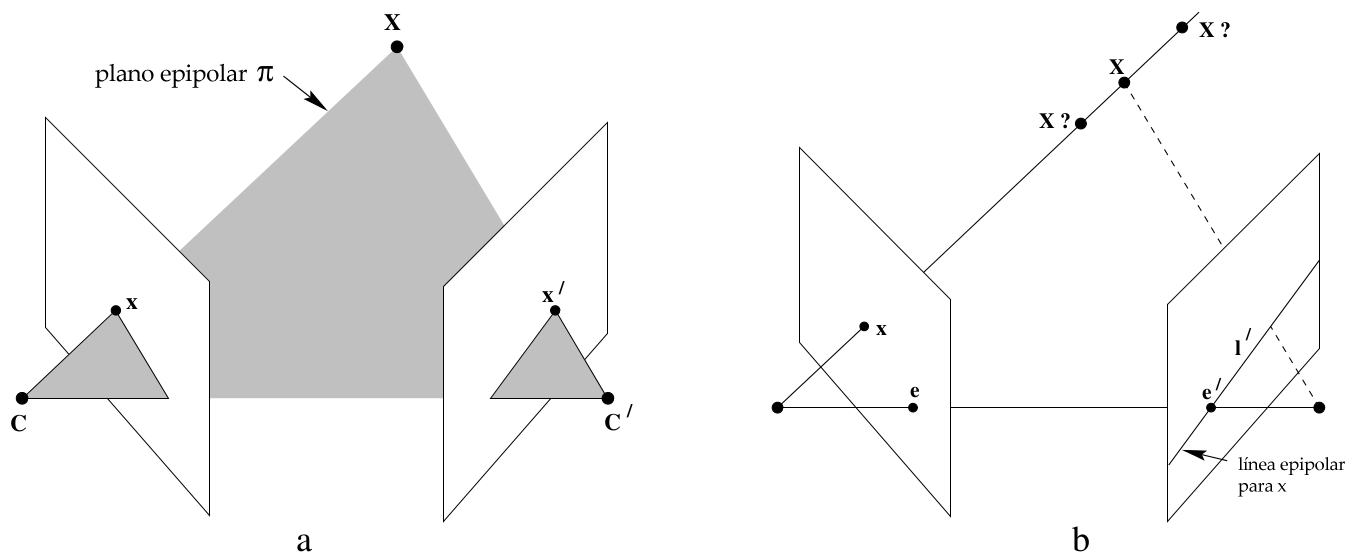
\includegraphics[width=1.0\textwidth]{images/pointcorrespgeom.png}
\caption[Geometr\'{i}a de correspondencia de puntos]%
{\textbf{(a)} Las dos c\'{a}maras son indicadas por sus centros \textbf{C} y \textbf{C'} y los planos de las im\'{a}genes. Los centros de las c\'{a}maras, el punto tridimensional \textbf{X} y sus im\'{a}genes \textbf{x} y \textbf{x'} se encuentran todos en un plano com\'{u}n \textbf{$\pi$}. \textbf{(b)} Un punto \textbf{x} de una imagen se retroproyecta hacia un rayo en un espacio tridimensional definido por el primer centro de la c\'{a}mara \textbf{C} y por \textbf{x}. Este rayo se representa como la l\'{i}nea \textbf{l'} en la segunda vista. El punto tridimensional \textbf{X}, el cual se proyecta hacia \textbf{x}, \underline{debe} encontrarse en este rayo, de manera que la imagen de \textbf{X} en la segunda vista debe encontrarse en \textbf{l'}. Imagen tomada del libro \textit{Multiple View Geometry} de Richard Hartley y Andrew Zisserman \copyright \cite{Hartley_Zisserman_2003}.}
\label{fig:PointCorrespondenceFGeometry}
\end{figure}


\begin{figure}[H]
\centering
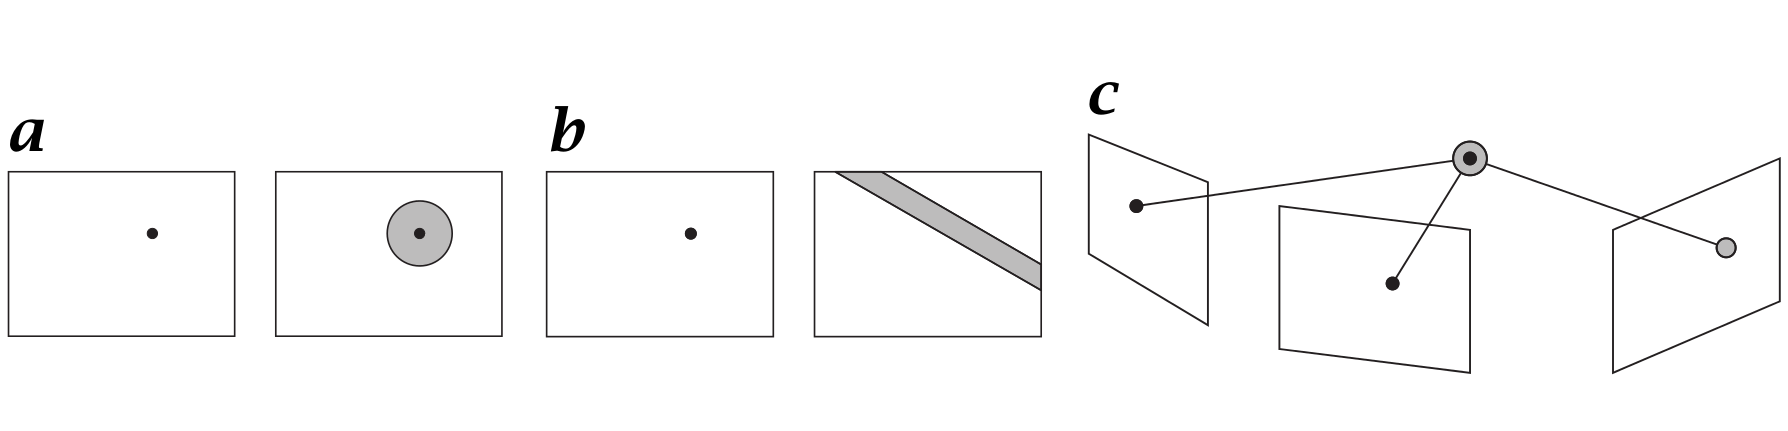
\includegraphics[width=1.0\textwidth]{images/searchregion1.png}
\caption[Restricci\'{o}n del \'{a}rea de b\'{u}squeda de puntos]%
{\textbf{(a)} Imagen con una regi\'{o}n de b\'{u}squeda estimada \textit{a priori}. \textbf{(b)} Regi\'{o}n de b\'{u}squeda estimada utilizando geometr\'{i}a epipolar. \textbf{(c)} Predicci\'{o}n de una regi\'{o}n de b\'{u}squeda despu\'{e}s de una reconstrucci\'{o}n proyectiva del punto (utilizada para refinamiento). Imagen tomada del libro \textit{Handbook of Computer Vision and Applications} de Jahne B. \copyright \cite{Jahne_Haussecker_Geibler_1999}.}
\label{fig:SearchRegion1}
\end{figure}


La matriz fundamental (ll\'{a}mese \textit{\textbf{F}}) encapsula la geometr\'{i}a epipolar la cual es necesaria para la reconstrucci\'{o}n. Se define como una matriz de 3x3 de rango 2 la cual determina la relaci\'{o}n que existe entre puntos clave en pares de im\'{a}genes estereosc\'{o}picas. Si un punto en el espacio tridimensional \textit{X} es proyectado como \textit{x} en la primera vista, y como \textit{x'} en la segunda vista, entonces los puntos de la imagen satisfacen la relaci\'{o}n $x'^TFx = 0$ \cite{Faugeras_1993,Shah_1983,Hartley_Zisserman_2003,Faugeras_Luong_2001}. Esto significa que utilizando geometr\'{i}a epipolar, es posible determinar la matriz fundamental a partir de correspondencia de puntos en pares de im\'{a}genes estereosc\'{o}picas. En \cite{Hartley_Zisserman_2003} se muestran diferentes t\'{e}cnicas para recuperar la matriz fundamental \textit{F} utilizando correspondencia de puntos y a su vez, se prueba que tanto la matriz de rotaci\'{o}n \textit{R} y como la de traslaci\'{o}n \textit{t} pueden ser inferidas a partir de \textit{F}.

Una de las t\'{e}cnicas m\'{a}s sugeridas para encontrar \textit{F} es el algoritmo de correspondencia de 7 puntos descrito en \cite{Faugeras_1993,Hartley_Zisserman_2003}. Pero dado que el mapa de movimiento estimado en la fase anterior permite determinar una cantidad mucho mayor de puntos clave, se opt\'{o} por utilizar la implementaci\'{o}n\footnote{Se utiliz\'{o} la implementaci\'{o}n que viene en la biblioteca de visi\'{o}n artificial conocida como OpenCV.} de un algoritmo m\'{a}s robusto basado en \textit{RANSAC} (del ingl\'{e}s \textit{RANdom SAmple Consensus}).

Publicado por Fischler y Bolles en 1981, se define como un algoritmo iterativo que permite estimar los par\'{a}metros de un modelo matem\'{a}tico a partir de un conjunto de datos observados en los cuales existen valores at\'{i}picos (del ingl\'{e}s \textit{outliers}) \cite{Fischler_Bolles_1981,Chum_2005}. RANSAC es utilizado a menudo en el \'{a}rea de la visi\'{o}n artificial para resolver simult\'{a}neamente el problema de correspondencia de puntos y el de estimaci\'{o}n de la matriz fundamental a partir de un par de im\'{a}genes estereosc\'{o}picas \cite{Forsyth_Ponce_2002,Hartley_Zisserman_2003,Torr_Murray_1997,Chum_2005}.


\begin{figure}[H]
\centering
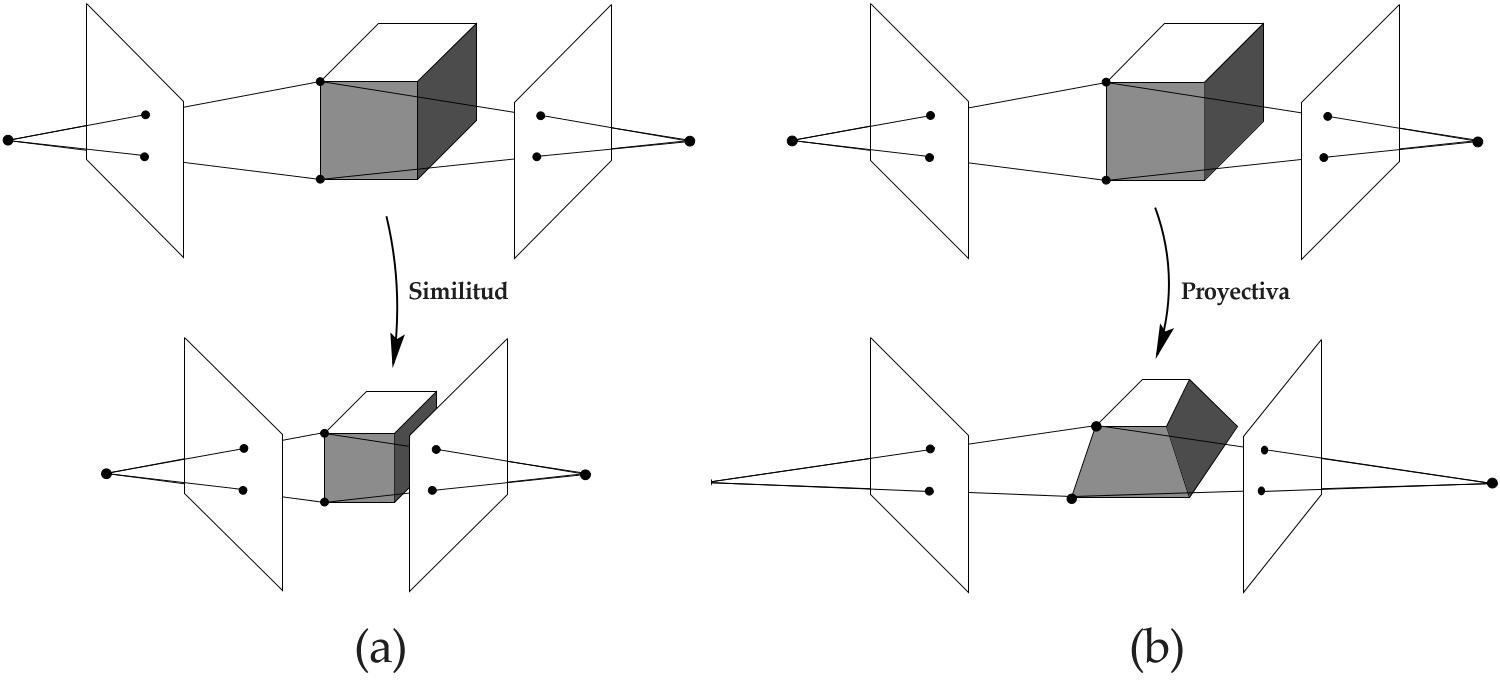
\includegraphics[width=1.0\textwidth]{images/projectiveambiguity1.png}
\caption[Problema de ambigüedad proyectiva]%
{\textbf{(a)} Si las c\'{a}maras est\'{a}n calibradas, cualquier reconstrucci\'{o}n debe respetar el \'{a}ngulo entre los rayos medidos en la imagen. Una transformaci\'{o}n de similitud de la estructura
y posiciones de c\'{a}mara no altera el \'{a}ngulo medido. El \'{a}ngulo entre los rayos y la l\'{i}nea base (epipolos) tampoco son alterados. \textbf{(b)} Si las c\'{a}maras no est\'{a}n calibradas, las reconstrucciones s\'{o}lo deben respetar los puntos de la imagen (la intersecci\'{o}n de los rayos con el plano de la imagen). Una transformaci\'{o}n proyectiva de la estructura y de las posiciones de la c\'{a}mara no altera los puntos medidos, aunque el \'{a}ngulo entre los rayos
s\'{i} es alterado. Los epipolos tampoco son alterados (intersecci\'{o}n con la l\'{i}nea de base). Imagen tomada del libro \textit{Multiple View Geometry} de Richard Hartley y Andrew Zisserman \copyright.}
\label{fig:ReconstructionAmbiguity}
\end{figure}


A pesar de que RANSAC permite encontrar la matriz fundamental, existe el problema de ambigüedad proyectiva que se muestra en la figura ~\ref{fig:ReconstructionAmbiguity}. Esto significa que la matriz obtenida podr\'{i}a no ser la real dado que es posible que haya sido afectada por una transformaci\'{o}n tridimensional proyectiva \cite{Hartley_Zisserman_2003}. Para lidiar con este problema, se necesita encontrar otra matriz conocida como la matriz esencial \textit{\textbf{E}} \cite{Longuet_Higgins_1981}, la cual es una matriz con caracter\'{i}sticas muy similares a la matriz fundamental con la excepci\'{o}n de que s\'{o}lo se utiliza en c\'{a}maras calibradas. Esto permite remover la ambigüedad proyectiva y a su vez, permite realizar una reconstrucci\'{o}n m\'{e}trica, lo cual significa que los puntos tridimensionales est\'{a}n sujetos a una escala verdadera y no a una de transformaci\'{o}n proyectiva \cite{Cyganek_Siebert_2009,Hartley_Zisserman_2003,Szeliski_2010}.

Similar a la matriz fundamental, la matriz esencial \textit{\textbf{E}} tiene una dimensi\'{o}n de 3x3 e impone restricciones entre un punto de una imagen y un punto en la otra imagen de manera que $x'Ex = 0$, donde \textit{x} es un punto en una imagen y \textit{x'} es el punto correspondiente en la otra imagen. Para el c\'{a}lculo de la matriz esencial \textit{E} se utiliz\'{o} la siguiente ecuaci\'{o}n descrita en \cite{Szeliski_2010,Hartley_Zisserman_2003}:


\vspace{5 mm}
\begin{center}
$\mathbf{E = K'^TFK}$
\end{center}
\vspace{5 mm}


Utilizando la ecuaci\'{o}n anterior, es posible determinar la matriz esencial \textit{\textbf{E}} a partir de la matriz de la calibraci\'{o}n de la c\'{a}mara \textit{\textbf{K}} y la matriz fundamental \textit{\textbf{F}}. Una vez obtenida \textit{\textbf{E}}, se necesita extraer el elemento de rotaci\'{o}n \textit{\textbf{R}} y el de traslaci\'{o}n \textit{\textbf{t}} que se encuentran contenidos en ella.

Cabe destacar que la matriz \textit{E} s\'{o}lo brinda una de las dos c\'{a}maras\footnote{Por simplicidad, el t\'{e}rmino c\'{a}mara o matrices de la c\'{a}mara se utiliza indistintamente.} necesarias para la reconstrucci\'{o}n. Para obtener la otra c\'{a}mara se procede a fijar (no rotaci\'{o}n ni traslaci\'{o}n) una de las c\'{a}maras (ll\'{a}mese \textit{\textbf{P}}) y luego se calcula el elemento de rotaci\'{o}n \textit{R} y traslaci\'{o}n \textit{t} de la otra c\'{a}mara (ll\'{a}mese \textit{\textbf{P'}}) con respecto a \'{e}sta. Esto significa que cualquier punto tridimensional que se obtenga a partir de este par de c\'{a}maras tendr\'{a} su primera c\'{a}mara ubicada en la coordenada origen (0,0,0) y su segunda c\'{a}mara estar\'{a} ubicada en \textit{t} \cite{hartley1997triangulation,Hartley_Zisserman_2003}.

Se utiliz\'{o} la t\'{e}cnica de decomposici\'{o}n en valores singulares (del ingl\'{e}s \textit{singular value decomposition}) \cite{Wang_Tsui_2000} en conjunto con el c\'{a}lculo de las cuatro soluciones para reconstrucci\'{o}n calibrada detallado en \cite{Hartley_Zisserman_2003} para extraer los elementos de rotaci\'{o}n y traslaci\'{o}n de la segunda c\'{a}mara.


\begin{figure}[H]
\centering
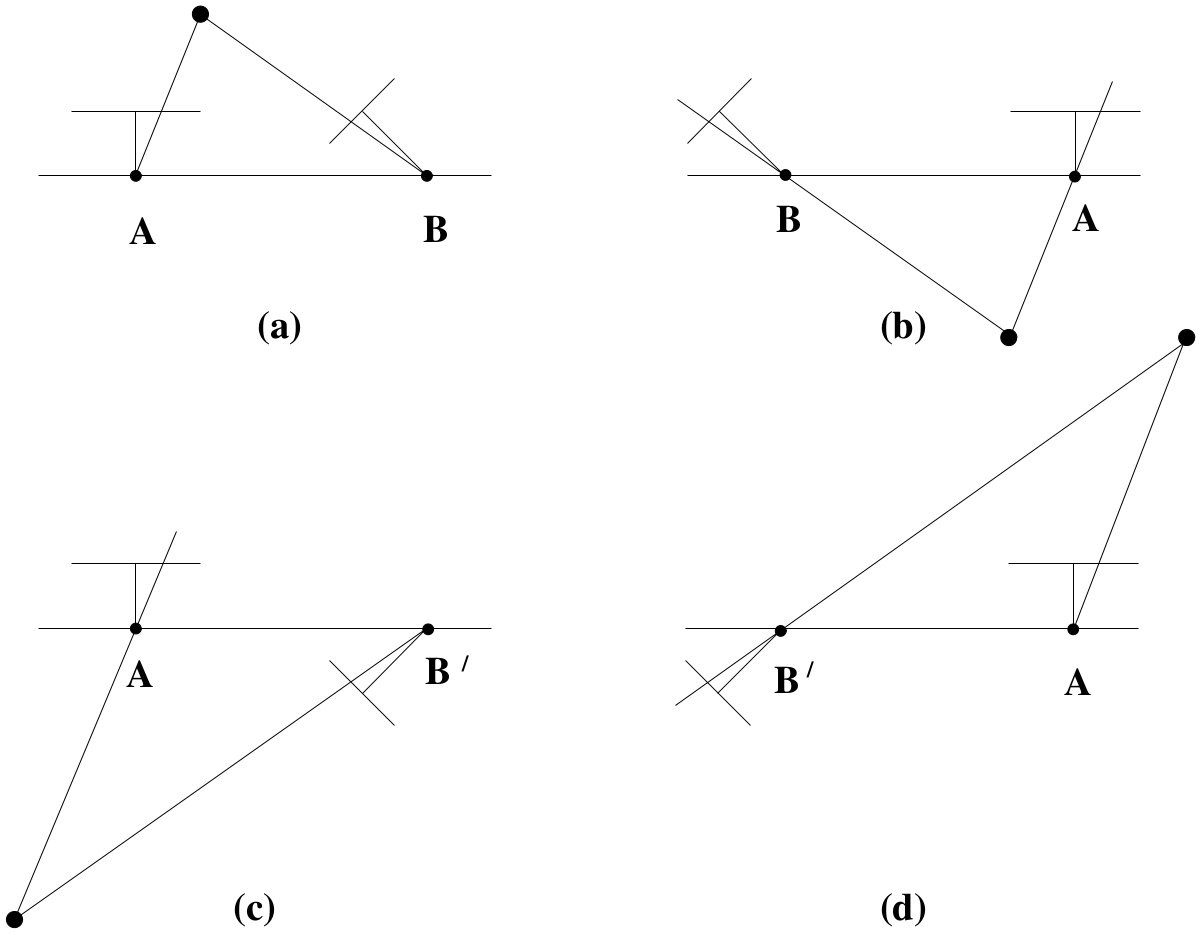
\includegraphics[width=1.0\textwidth]{images/foursolution1.png}
\caption[Cuatro posibles soluciones para reconstrucci\'{o}n calibrada usando \textit{E}]%
{Entre los lados izquierdo y derecho existe una inversi\'{o}n de la l\'{i}nea base. Entre las filas de arriba y abajo la c\'{a}mara \textit{B} rota $180^\circ$ sobre la l\'{i}nea base. N\'{o}tese que s\'{o}lo \textbf{(a)} es la reconstrucci\'{o}n del punto cuando \'{e}ste se encuentra frente a ambas c\'{a}maras. Imagen tomada del libro \textit{Multiple View Geometry} de Richard Hartley y Andrew Zisserman \copyright.}
\label{fig:FourSolutions1}
\end{figure}

Las cuatro posibles soluciones se ilustran en la figura ~\ref{fig:FourSolutions1}, donde se muestra que un punto reconstruido \textit{X} estar\'{a} frente a ambas c\'{a}maras solamente en una de cuatro las soluciones. De \'{e}sta forma basta probar con un solo punto para determinar si est\'{a} frente a ambas c\'{a}maras y as\'{i} decidir entre las cuatro diferentes soluciones para la matriz de la c\'{a}mara \textit{P'} \cite{Hartley_Zisserman_2003}.

El siguiente paso en la t\'{e}cnica es utilizar las matrices estimadas ($P$ y $P'$) de la c\'{a}mara para calcular la distancia de los puntos del objeto a reconstruir. A esta fase se le conoce como estimaci\'{o}n de la profundidad.

%@TODO resumen del capitulo